\section{GRU - Gated Recurrent Unit}
\begin{frame}{GRU - Gated Recurrent Unit}
  \LARGE GRU : \textbf{Gated Recurrent Unit}
\end{frame}

\begin{frame}{GRU - Gated Recurrent Unit}
  \small
  \textbf{Introduced by Cho et al., 2014}\\[0.8em]
  \textbf{Core Idea:} GRU uses \textbf{gates} to control what to keep, forget, and output.

  \vspace{1em}
  \textbf{Key Components:}
  \begin{itemize}
    \item[\textcolor{red}{$\blacktriangleright$}] \textbf{Update Gate} $z_t$
    \item[\textcolor{red}{$\blacktriangleright$}] \textbf{Reset Gate} $r_t$
  \end{itemize}
\end{frame}

\begin{frame}{GRU - Gated Recurrent Unit: Equations}
  \textbf{Equations:}
  \vspace{0.7em}

  \begin{align*}
    z_t &= \sigma(W_z[x_t, h_{t-1}] + b_z) \\
    r_t &= \sigma(W_r[x_t, h_{t-1}] + b_r) \\
    \tilde{h}_t &= \tanh(W_h[x_t, r_t * h_{t-1}] + b_h) \\
    h_t &= (1 - z_t) * h_{t-1} + z_t * \tilde{h}_t
  \end{align*}

  \vspace{1.5em}
  
  {\color{blue} \textbf{Comparable performance to LSTM}} \\
  {\color{blue} \textbf{Faster training, fewer parameters}}
\end{frame}

\begin{frame}{GRU - Gated Recurrent Units}
  \centering
  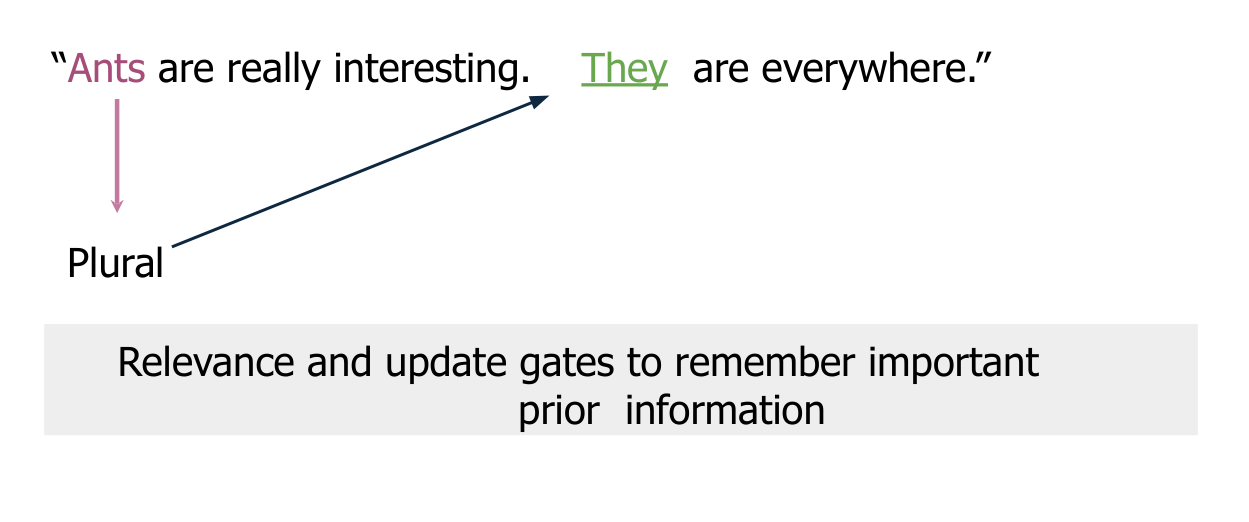
\includegraphics[width=0.9\paperwidth,height=0.95\paperheight,keepaspectratio]{assets/Lecture-3_Recurrent_Neural_Networks/pdf_page_072.png}
\end{frame}

\begin{frame}{GRU - Gated Recurrent Unit}
  \centering
  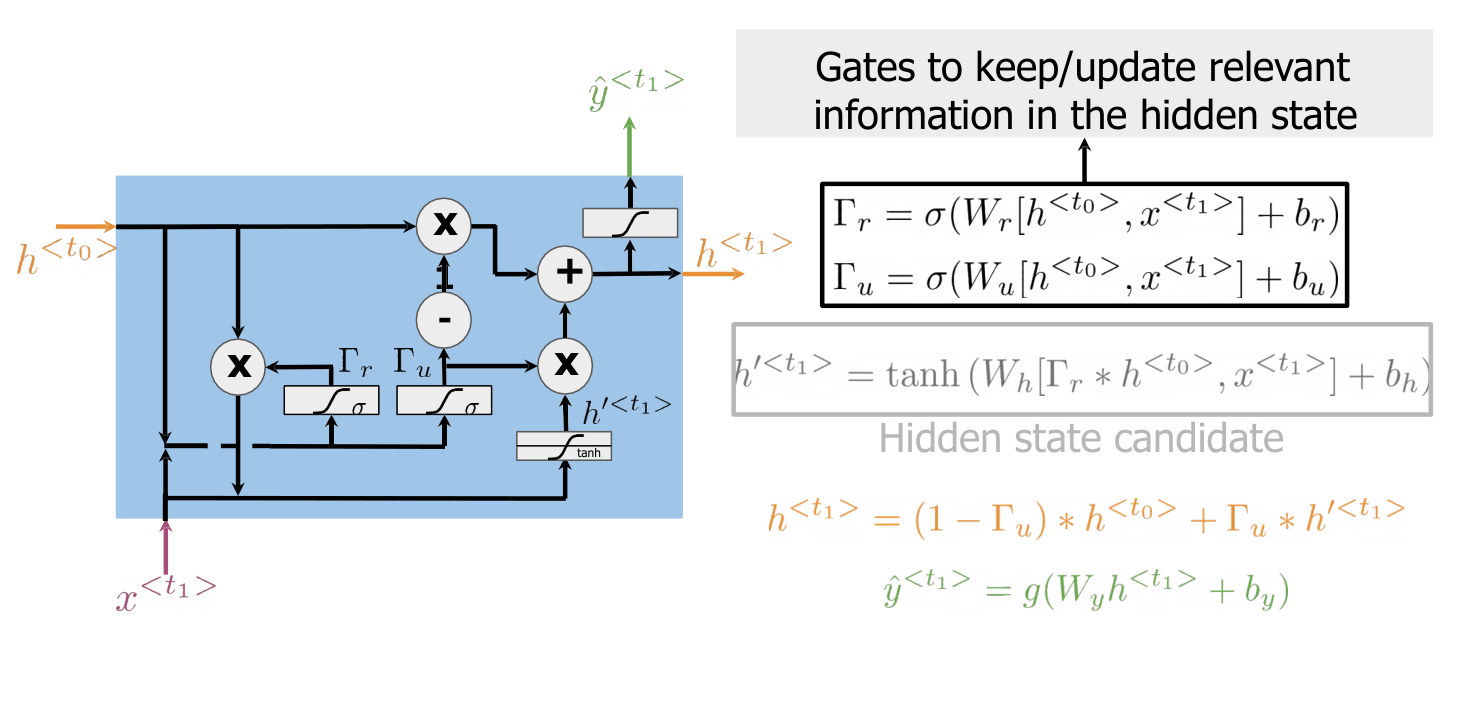
\includegraphics[width=0.9\paperwidth,height=0.95\paperheight,keepaspectratio]{assets/Lecture-3_Recurrent_Neural_Networks/pdf_page_073.png}
\end{frame}

\begin{frame}{Vanilla RNN vs GRUs}
  \centering
  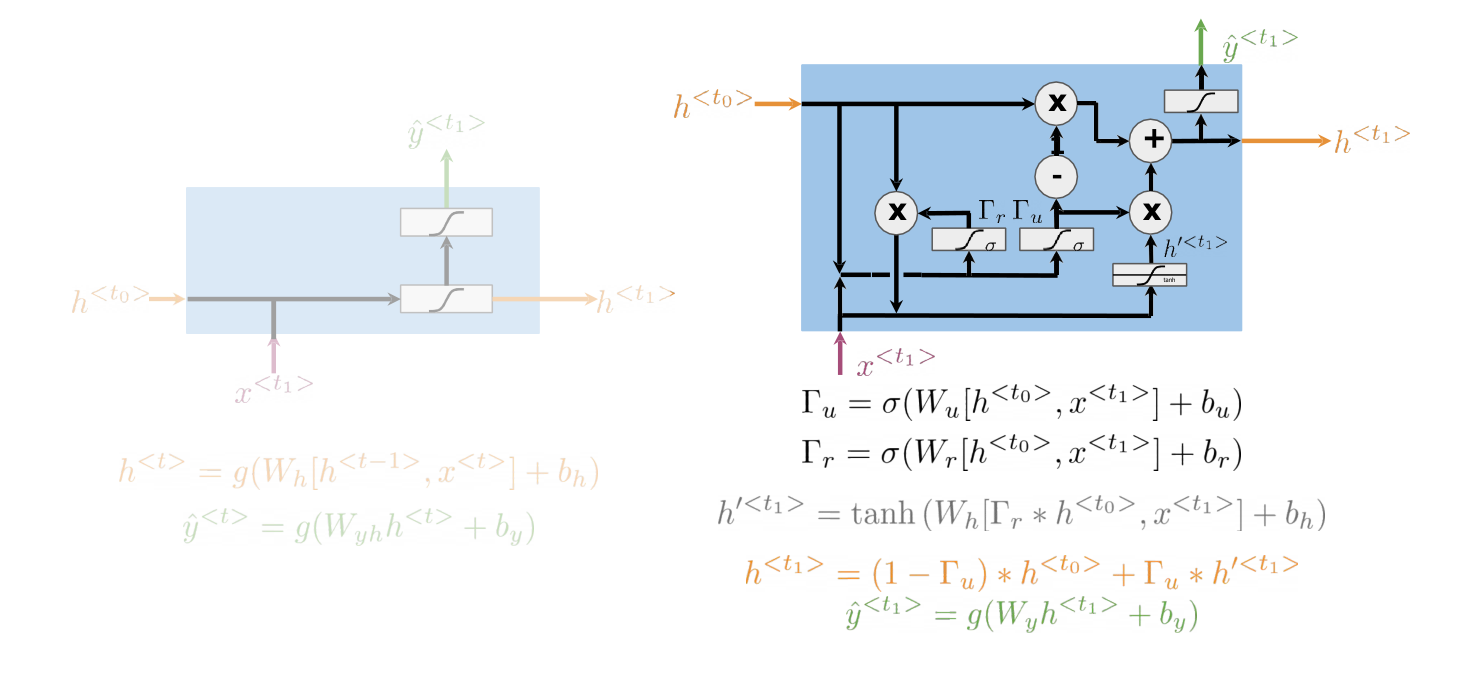
\includegraphics[width=0.9\paperwidth,height=0.95\paperheight,keepaspectratio]{assets/Lecture-3_Recurrent_Neural_Networks/pdf_page_074.png}
\end{frame}
